\hypertarget{redes-e-protocolos-de-comunicauxe7uxe3o-industrial}{%
\chapter{Redes e Protocolos de Comunicação Industrial}\label{redes-e-protocolos-de-comunicauxe7uxe3o-industrial}}

\section*{Objetivos de Aprendizagem}

Ao final deste capítulo, o leitor será capaz de:

\begin{itemize}
\tightlist
\item
  Identificar os principais protocolos de comunicação industrial e suas características.
\item
  Distinguir protocolos clássicos (Modbus, Profibus) de protocolos modernos (OPC UA, MQTT).
\item
  Compreender o papel de cada protocolo na arquitetura de um sistema SCADA.
\item
  Aplicar critérios técnicos para seleção de protocolo em projetos de automação.
\end{itemize}

\begin{center}\rule{0.5\linewidth}{0.5pt}\end{center}

\hypertarget{redes-industriais-versus-redes-corporativas}{%
\section{Redes Industriais versus Redes Corporativas}\label{redes-industriais-versus-redes-corporativas}}

As redes industriais possuem requisitos distintos das redes corporativas de TI:

\textbf{Tabela 5.1 -- Comparativo: Rede Corporativa \ensuremath{\times} Rede Industrial}

\begin{longtable}[]{@{}
  >{\raggedright\arraybackslash}p{(\columnwidth - 4\tabcolsep) * \real{0.3333}}
  >{\raggedright\arraybackslash}p{(\columnwidth - 4\tabcolsep) * \real{0.3333}}
  >{\raggedright\arraybackslash}p{(\columnwidth - 4\tabcolsep) * \real{0.3333}}@{}}
\toprule\noalign{}
\begin{minipage}[b]{\linewidth}\raggedright
Critério
\end{minipage} & \begin{minipage}[b]{\linewidth}\raggedright
Rede Corporativa (TI)
\end{minipage} & \begin{minipage}[b]{\linewidth}\raggedright
Rede Industrial (OT)
\end{minipage} \\
\midrule\noalign{}
\endhead
\bottomrule\noalign{}
\endlastfoot
Prioridade & Confidencialidade, disponibilidade & Determinismo, tempo real \\
Latência & Tolerável (ms a s) & Crítica (\ensuremath{\mu}s a ms) \\
Disponibilidade & Alta (99,9\%) & Muito alta (99,999\%) \\
Equipamentos & PCs, servidores, switches & CLPs, RTUs, inversores, sensores \\
Ambiente & Sala climatizada & Calor, vibração, poeira, EMI \\
Ciclo de vida & 3--5 anos & 10--30 anos \\
Atualização & Frequente & Raramente (risco de parada) \\
\end{longtable}

\begin{caixaatencao}

\textbf{Atenção:} A convergência TI/OT é inevitável com o IIoT, mas deve ser feita com cuidado. Trazer protocolos e infraestrutura de TI (ex.: Wi-Fi público, VLAN sem segmentação) para o ambiente OT sem as devidas proteções é a principal causa de incidentes de segurança industrial. Ver Capítulo 8.

\end{caixaatencao}

\begin{center}\rule{0.5\linewidth}{0.5pt}\end{center}

\hypertarget{modelo-osi-aplicado-uxe0-automauxe7uxe3o}{%
\section{Modelo OSI Aplicado à Automação}\label{modelo-osi-aplicado-uxe0-automauxe7uxe3o}}

O modelo \textbf{OSI} (\emph{Open Systems Interconnection}) de 7 camadas é frequentemente referenciado para classificar os protocolos industriais:

\begin{center}
\IfFileExists{../figuras/capitulo-05-m1.pdf}{%
  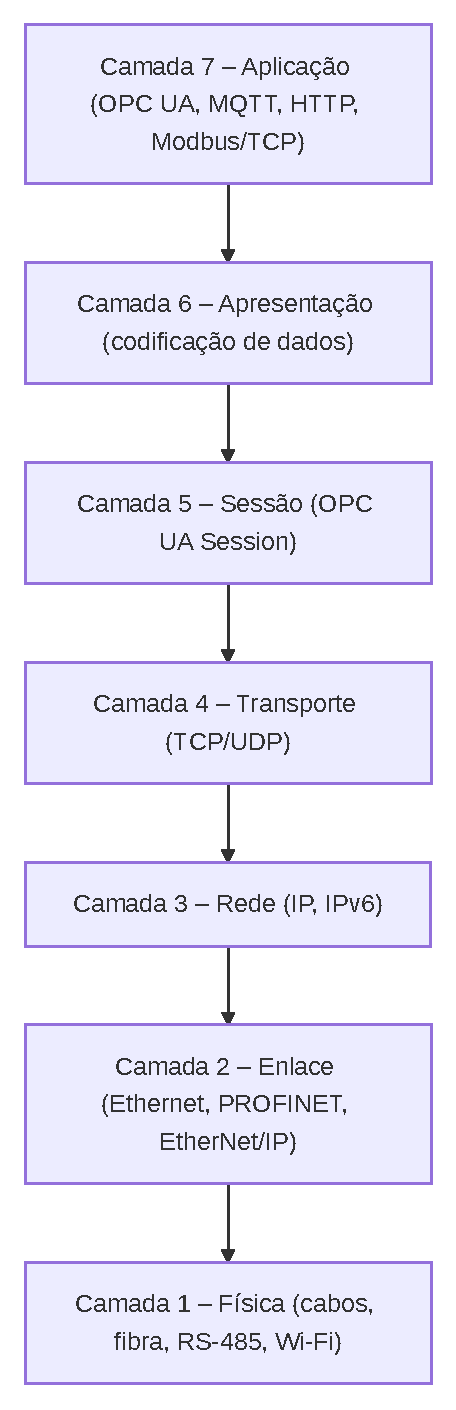
\includegraphics[width=\linewidth,height=0.8\textheight,keepaspectratio]{../figuras/capitulo-05-m1.pdf}%
}{\fbox{\parbox{0.9\linewidth}{\small Diagrama Mermaid ainda não renderizado: capitulo-05-m1. Rode scripts/render-mermaid.sh.}}}
\end{center}

\begin{caixafigura}

\textbf{{[}Figura 5.1 -- Protocolos industriais mapeados no modelo OSI{]}}
\emph{Diagrama de 7 camadas OSI com protocolos industriais posicionados nas camadas correspondentes. Destacar: Modbus RTU (camadas 1-2), Modbus TCP (completo), OPC UA (7), MQTT (7), Profibus (1-2-7), PROFINET (1-2-7).}

\end{caixafigura}

\begin{center}\rule{0.5\linewidth}{0.5pt}\end{center}

\hypertarget{protocolos-cluxe1ssicos}{%
\section{Protocolos Clássicos}\label{protocolos-cluxe1ssicos}}

\hypertarget{modbus}{%
\subsection{Modbus}\label{modbus}}

O \textbf{Modbus} foi criado pela Modicon em 1979 e é um dos protocolos mais simples e amplamente suportados no mundo. Sua popularidade se deve à especificação aberta, gratuita e fácil de implementar.

\textbf{Variantes:}
- \textbf{Modbus RTU:} comunicação serial (RS-232 ou RS-485), codificação binária compacta. Máximo de 247 escravos por barramento RS-485.
- \textbf{Modbus ASCII:} comunicação serial, codificação hexadecimal. Raramente usado hoje.
- \textbf{Modbus TCP/IP:} encapsula o Modbus RTU sobre TCP, na porta 502. Permite comunicação via Ethernet com distâncias ilimitadas.

\textbf{Modelo de dados Modbus:}

\begin{longtable}[]{@{}
  >{\raggedright\arraybackslash}p{(\columnwidth - 6\tabcolsep) * \real{0.2500}}
  >{\raggedright\arraybackslash}p{(\columnwidth - 6\tabcolsep) * \real{0.2500}}
  >{\raggedright\arraybackslash}p{(\columnwidth - 6\tabcolsep) * \real{0.2500}}
  >{\raggedright\arraybackslash}p{(\columnwidth - 6\tabcolsep) * \real{0.2500}}@{}}
\toprule\noalign{}
\begin{minipage}[b]{\linewidth}\raggedright
Área
\end{minipage} & \begin{minipage}[b]{\linewidth}\raggedright
Tipo
\end{minipage} & \begin{minipage}[b]{\linewidth}\raggedright
Acesso
\end{minipage} & \begin{minipage}[b]{\linewidth}\raggedright
Exemplo
\end{minipage} \\
\midrule\noalign{}
\endhead
\bottomrule\noalign{}
\endlastfoot
Coils (0x) & Bit & Leitura/Escrita & Status de válvula, partida de motor \\
Discrete Inputs (1x) & Bit & Somente Leitura & Estado de botoeira, fim de curso \\
Holding Registers (4x) & Word 16 bits & Leitura/Escrita & Setpoint de temperatura, referência de velocidade \\
Input Registers (3x) & Word 16 bits & Somente Leitura & Valor de temperatura, corrente de motor \\
\end{longtable}

\begin{caixadica}

\textbf{Dica:} Para representar valores de ponto flutuante (ex.: 25,4\ensuremath{^\circ}C) em Modbus, utiliza-se 2 registradores consecutivos de 16 bits no formato \textbf{IEEE 754} (32 bits). A ordem dos bytes (\emph{byte order} ou \emph{endianness}) varia por fabricante --- sempre verifique na documentação do equipamento.

\end{caixadica}

\begin{figure}
\centering
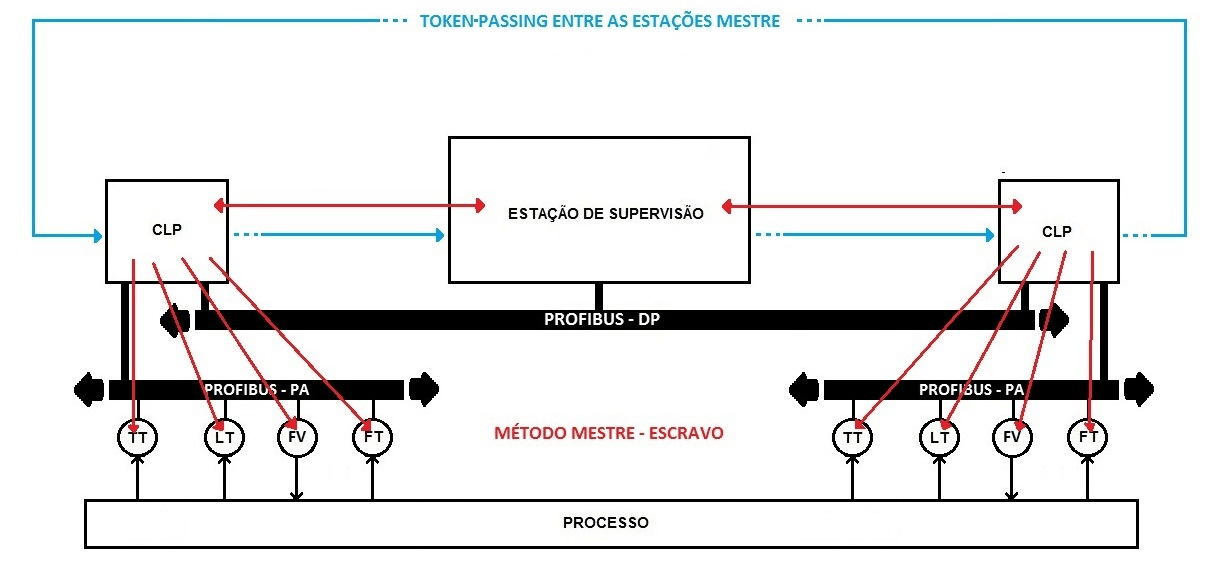
\includegraphics{../figuras/cap05-mestre-escravo-token.png}
\caption[Figura 5.2 -- Métodos de acesso ao meio: mestre-escravo e token passing]{Figura 5.2 -- Métodos de acesso ao meio: mestre-escravo e token passing. \textbf{Fonte:} \emph{Livro SCADA --- versão para análise}, p.~31 (Machado, Pontes e Vianna, reproduzida com crédito).}
\end{figure}

No método \textbf{mestre-escravo}, o mestre conduz a comunicação e cada instrumento responde quando
interrogado --- é o modelo do Modbus RTU. No \textbf{token passing}, o direito de transmitir circula entre
as estações mestre por um quadro especial, o que evita colisão sem precisar de um mestre único.

\hypertarget{profibus}{%
\subsection{Profibus}\label{profibus}}

O \textbf{Profibus} (\emph{Process Field Bus}) foi desenvolvido na Alemanha em 1987 e tornou-se o protocolo de fieldbus mais utilizado na Europa para automação discreta e de processo.

\textbf{Variantes:}
- \textbf{Profibus DP} (\emph{Decentralized Peripherals}): otimizado para comunicação rápida com CLPs e módulos de I/O distribuído. Velocidades até 12 Mbps.
- \textbf{Profibus PA} (\emph{Process Automation}): para instrumentação de processo em zonas de risco (alimentação e comunicação pelo mesmo par de fios --- barramento intrínseco).

\textbf{Limitações:} padrão aberto e publicado (séries IEC 61158/61784), mas com certificação obrigatória
para conformidade; não trafega nativamente sobre IP --- a evolução sobre Ethernet é o \textbf{PROFINET};
e o diagnóstico é menos imediato que o de uma rede IP.

\hypertarget{dnp3}{%
\subsection{DNP3}\label{dnp3}}

O \textbf{DNP3} (\emph{Distributed Network Protocol 3}) foi desenvolvido para sistemas SCADA de infraestrutura crítica --- energia elétrica, água, óleo e gás. Características:

\begin{itemize}
\tightlist
\item
  Comunicação assíncrona: RTU reporta espontaneamente ao mestre quando uma variável muda (\emph{unsolicited response}) --- diferente do polling periódico do Modbus.
\item
  Suporte a \textbf{time-stamping} preciso nos eventos --- crucial para análise de incidentes em subestações.
\item
  Suporte a comunicação com integridade de dados e autenticação (DNP3 Secure Authentication v5).
\item
  Norma IEEE Std 1815-2012.
\end{itemize}

\hypertarget{foundation-fieldbus}{%
\subsection{Foundation Fieldbus}\label{foundation-fieldbus}}

O \textbf{Foundation Fieldbus} (FF) leva a lógica de controle para dentro do próprio barramento: os
instrumentos são inteligentes, comunicam-se entre si e podem executar blocos de controle sem
passar pelo CLP. Como não existe um mestre único, o direito de uso do meio é arbitrado pelo
\textbf{LAS} (\emph{Link Active Scheduler}), que distribui as janelas de tempo entre as estações.

\begin{figure}
\centering
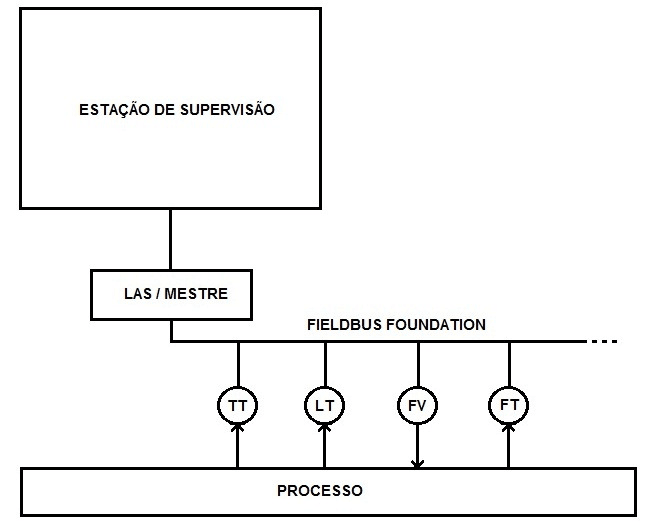
\includegraphics{../figuras/cap05-fieldbus-foundation.png}
\caption[Figura 5.3 -- Arquitetura com Foundation Fieldbus]{Figura 5.3 -- Arquitetura com Foundation Fieldbus. \textbf{Fonte:} \emph{Livro SCADA --- versão para análise}, p.~29 (Machado, Pontes e Vianna, reproduzida com crédito).}
\end{figure}

O LAS \textbf{não} é um mestre no sentido do Modbus: ele agenda \emph{quando} cada dispositivo pode falar,
e outro instrumento habilitado pode assumir a função de LAS ativo se o original falhar. Os
transmissores da figura (TT, LT, FV, FT) ligam-se ao mesmo par que os alimenta --- característica
que viabiliza o uso do FF em áreas classificadas, onde a alimentação intrinsecamente segura e a
comunicação precisam compartilhar o cabo.

\begin{center}\rule{0.5\linewidth}{0.5pt}\end{center}

\hypertarget{protocolos-modernos}{%
\section{Protocolos Modernos}\label{protocolos-modernos}}

\hypertarget{opc-e-opc-ua}{%
\subsection{OPC e OPC UA}\label{opc-e-opc-ua}}

O \textbf{OPC} (\emph{OLE for Process Control}) surgiu em 1996 como padrão de interoperabilidade entre softwares SCADA e CLPs no ambiente Windows. O problema: dependia fortemente de tecnologia Microsoft COM/DCOM, limitando seu uso a redes Windows.

O \textbf{OPC UA} (\emph{Unified Architecture}), lançado em 2008 pela OPC Foundation, resolve essas limitações:

\begin{itemize}
\tightlist
\item
  \textbf{Plataforma-independente:} funciona em Linux, embarcados, CLPs modernos --- não mais dependente de Windows.
\item
  \textbf{Modelo de informação orientado a objetos:} dados são expostos como objetos com tipos, métodos e eventos --- muito mais rico que endereços de registradores.
\item
  \textbf{Segurança nativa:} TLS/SSL e assinatura de certificados embutidos no protocolo.
\item
  \textbf{Transporte flexível:} TCP binário (eficiente) ou HTTPS/WebSocket (firewall-friendly).
\item
  \textbf{Publisher-Subscriber:} adicionado no OPC UA Pub/Sub, permitindo comunicação via MQTT ou UDP multicast --- integração nativa com IIoT.
\end{itemize}

\begin{center}
\IfFileExists{../figuras/capitulo-05-m2.pdf}{%
  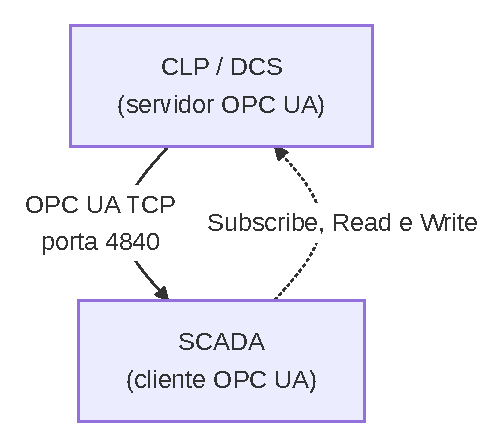
\includegraphics[width=\linewidth,height=0.8\textheight,keepaspectratio]{../figuras/capitulo-05-m2.pdf}%
}{\fbox{\parbox{0.9\linewidth}{\small Diagrama Mermaid ainda não renderizado: capitulo-05-m2. Rode scripts/render-mermaid.sh.}}}
\end{center}

\begin{caixafigura}

\textbf{{[}Figura 5.4 -- Arquitetura OPC UA: servidor no CLP, cliente no SCADA{]}}
\emph{Diagrama mostrando CLP com OPC UA Server integrado, conectado via rede Ethernet ao servidor SCADA (OPC UA Client). Indicar as operações: Read, Write, Subscribe, Browse. Destacar o certificado de segurança na conexão.}

\end{caixafigura}

\begin{caixanota}

\textbf{Nota:} O OPC UA é hoje o protocolo preferido para integração SCADA-CLP em novos projetos. Todos os grandes fabricantes de CLP (Siemens, Rockwell, Beckhoff, Schneider) oferecem servidores OPC UA nativos em seus equipamentos.

\end{caixanota}

\hypertarget{mqtt}{%
\subsection{MQTT}\label{mqtt}}

O \textbf{MQTT} (\emph{Message Queuing Telemetry Transport}) foi criado em 1999 pela IBM para telemetria em oleodutos via satélite --- com requisitos de baixo consumo de banda. Hoje é o protocolo dominante para IIoT.

\textbf{Arquitetura Publish-Subscribe:}

\begin{center}
\IfFileExists{../figuras/capitulo-05-m3.pdf}{%
  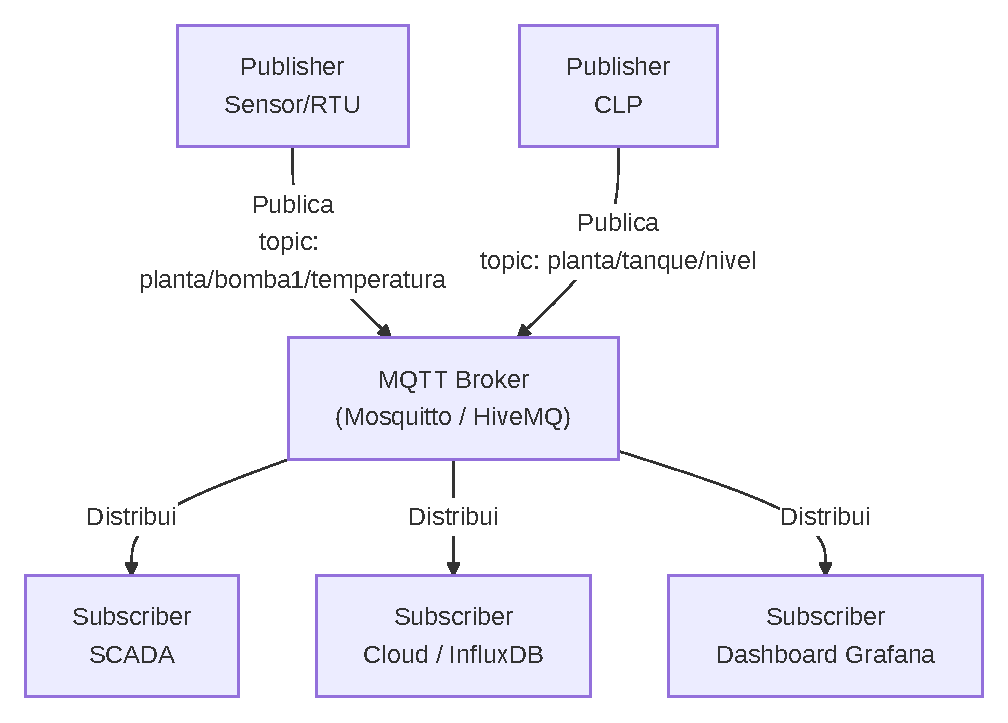
\includegraphics[width=\linewidth,height=0.8\textheight,keepaspectratio]{../figuras/capitulo-05-m3.pdf}%
}{\fbox{\parbox{0.9\linewidth}{\small Diagrama Mermaid ainda não renderizado: capitulo-05-m3. Rode scripts/render-mermaid.sh.}}}
\end{center}

\begin{caixafigura}

\textbf{{[}Figura 5.5 -- Modelo Publish-Subscribe do MQTT{]}}
\emph{Diagrama colorido mostrando múltiplos publishers (CLPs, sensores IIoT, edge gateways) publicando em um broker central (mosquitto). Múltiplos subscribers (SCADA, banco de dados, dashboards, mobile app) recebendo dados por tópicos. Destacar a escalabilidade horizontal.}

\end{caixafigura}

\textbf{Características técnicas:}
- Leve: overhead mínimo (cabeçalho de 2 bytes) --- ideal para dispositivos com memória e banda limitadas.
- \textbf{QoS} (\emph{Quality of Service}): 3 níveis: 0 (at-most-once), 1 (at-least-once), 2 (exactly-once).
- \textbf{Retained messages:} o broker armazena o último valor de cada tópico; novos subscribers recebem imediatamente.
- \textbf{Last Will and Testament (LWT):} mensagem publicada automaticamente se o cliente desconectar inesperadamente --- mecanismo de detecção de falha.
- Porta padrão: 1883 (TCP) ou 8883 (TLS).
- \textbf{Sparkplug B:} especificação sobre MQTT com esquema de dados padronizado para IIoT industrial --- define payloads, timestamps e gerenciamento de sessão.

\textbf{Brokers MQTT populares:}
- \textbf{Mosquitto} (Eclipse Foundation) --- open-source, leve, amplamente usado.
- \textbf{HiveMQ} --- enterprise, alta escalabilidade, clustering.
- \textbf{EMQX} --- alta performance, suporte a MQTT 5.0.
- \textbf{AWS IoT Core, Azure IoT Hub} --- brokers gerenciados na nuvem.

\hypertarget{profinet}{%
\subsection{PROFINET}\label{profinet}}

O \textbf{PROFINET} é o sucessor do Profibus para redes Ethernet industrial, desenvolvido pela Siemens e padronizado pela PI (PROFIBUS \& PROFINET International).

\begin{itemize}
\tightlist
\item
  \textbf{PROFINET RT} (\emph{Real-Time}): para I/O distribuído --- ciclos de 1--4 ms.
\item
  \textbf{PROFINET IRT} (\emph{Isochronous Real-Time}): para motion control --- ciclos de 250 \ensuremath{\mu}s com sincronismo de relógio.
\item
  Compatível com infraestrutura Ethernet padrão (switches, cabos Cat5e/6).
\end{itemize}

\hypertarget{ethernetip}{%
\subsection{EtherNet/IP}\label{ethernetip}}

O \textbf{EtherNet/IP} (\emph{Ethernet Industrial Protocol}) é o protocolo da Rockwell Automation e ODVA para automação discreta. Usa o protocolo CIP (\emph{Common Industrial Protocol}) encapsulado em TCP/UDP/IP. Muito utilizado no ecossistema Allen-Bradley.

\begin{center}\rule{0.5\linewidth}{0.5pt}\end{center}

\hypertarget{comparativo-de-protocolos}{%
\section{Comparativo de Protocolos}\label{comparativo-de-protocolos}}

\textbf{Tabela 5.2 -- Principais protocolos industriais: comparativo}

\begin{longtable}[]{@{}
  >{\raggedright\arraybackslash}p{(\columnwidth - 10\tabcolsep) * \real{0.1667}}
  >{\raggedright\arraybackslash}p{(\columnwidth - 10\tabcolsep) * \real{0.1667}}
  >{\raggedright\arraybackslash}p{(\columnwidth - 10\tabcolsep) * \real{0.1667}}
  >{\raggedright\arraybackslash}p{(\columnwidth - 10\tabcolsep) * \real{0.1667}}
  >{\raggedright\arraybackslash}p{(\columnwidth - 10\tabcolsep) * \real{0.1667}}
  >{\raggedright\arraybackslash}p{(\columnwidth - 10\tabcolsep) * \real{0.1667}}@{}}
\toprule\noalign{}
\begin{minipage}[b]{\linewidth}\raggedright
Protocolo
\end{minipage} & \begin{minipage}[b]{\linewidth}\raggedright
Camada Física
\end{minipage} & \begin{minipage}[b]{\linewidth}\raggedright
Topologia
\end{minipage} & \begin{minipage}[b]{\linewidth}\raggedright
Velocidade
\end{minipage} & \begin{minipage}[b]{\linewidth}\raggedright
Segurança
\end{minipage} & \begin{minipage}[b]{\linewidth}\raggedright
Aplicação Principal
\end{minipage} \\
\midrule\noalign{}
\endhead
\bottomrule\noalign{}
\endlastfoot
Modbus RTU & RS-485 & Barramento & 9,6k--115,2 kbps & Nenhuma nativa & CLP instrumento \\
Modbus TCP & Ethernet & Estrela/Anel & 10/100 Mbps & Opcional (TLS) & CLP SCADA \\
Profibus DP & RS-485 & Barramento & até 12 Mbps & Nenhuma & Automação discreta EU \\
DNP3 & Serial / TCP & Barramento / Estrela & variável & SAv5 opcional & SCADA energia/água \\
OPC DA & Ethernet (DCOM) & Estrela & variável & Windows DCOM & SCADA legado Windows \\
\textbf{OPC UA} & Ethernet / qualquer & Qualquer & variável & TLS + certificado & SCADA moderno, IIoT \\
\textbf{MQTT} & Ethernet / 4G / Wi-Fi & Pub/Sub (broker) & variável & TLS opcional & IIoT, telemetria, cloud \\
PROFINET & Ethernet & Estrela/Anel & 100 Mbps & Opcional & I/O distribuído Siemens \\
EtherNet/IP & Ethernet & Estrela & 100 Mbps / 1 Gbps & CIPsecurity & I/O Rockwell/AB \\
\end{longtable}

\begin{center}\rule{0.5\linewidth}{0.5pt}\end{center}

\hypertarget{estudo-de-caso-integrauxe7uxe3o-modbus-opc-ua-mqtt}{%
\section{\texorpdfstring{Estudo de Caso --- Integração Modbus + OPC UA + MQTT}{Estudo de Caso  Integração Modbus + OPC UA + MQTT}}\label{estudo-de-caso-integrauxe7uxe3o-modbus-opc-ua-mqtt}}

\textbf{Contexto:} Uma planta química possui CLPs Siemens S7-1500 (OPC UA nativo) e instrumentos de campo com Modbus RTU (transmissores antigos sem Ethernet).

\textbf{Solução de integração:}

\begin{center}
\IfFileExists{../figuras/capitulo-05-m4.pdf}{%
  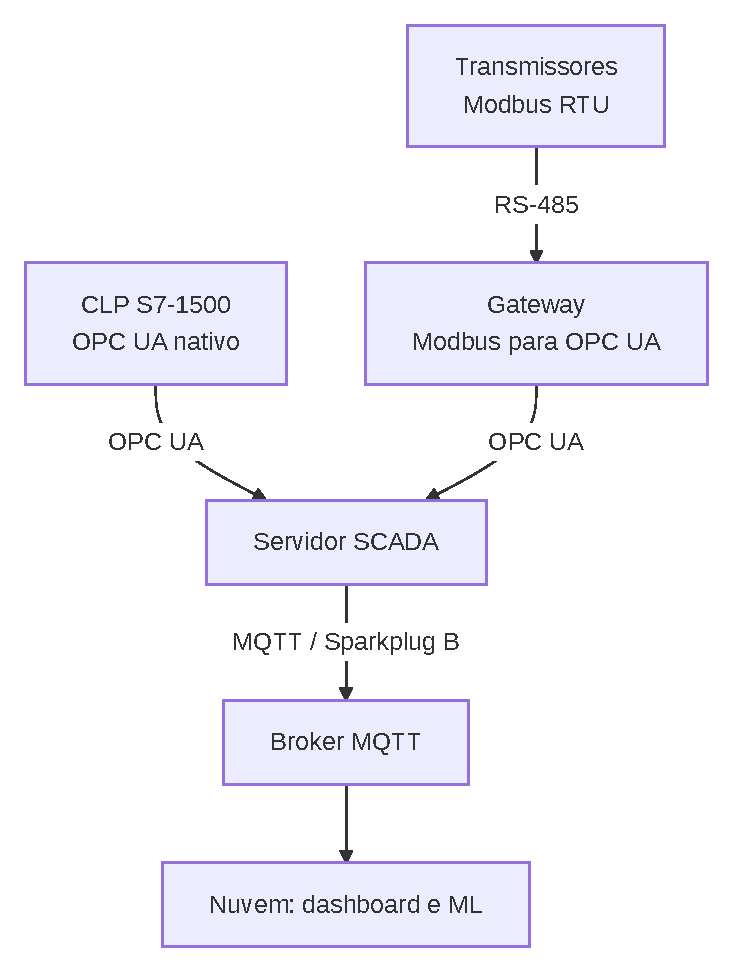
\includegraphics[width=\linewidth,height=0.8\textheight,keepaspectratio]{../figuras/capitulo-05-m4.pdf}%
}{\fbox{\parbox{0.9\linewidth}{\small Diagrama Mermaid ainda não renderizado: capitulo-05-m4. Rode scripts/render-mermaid.sh.}}}
\end{center}

\begin{figure}
\centering
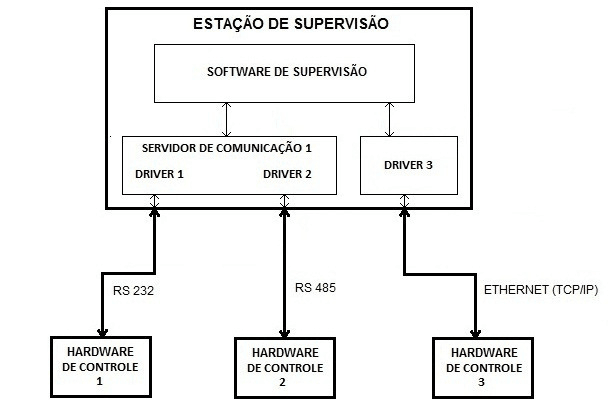
\includegraphics{../figuras/cap05-servidor-driver.png}
\caption[Figura 5.6 -- Integração de múltiplos protocolos em um servidor de supervisão]{Figura 5.6 -- Integração de múltiplos protocolos em um servidor de supervisão. \textbf{Fonte:} \emph{Livro SCADA --- versão para análise}, p.~25 (Machado, Pontes e Vianna, reproduzida com crédito).}
\end{figure}

O software de supervisão não fala ``Modbus'' nem ``PROFIBUS'': ele conversa com \textbf{drivers}. Na
figura, três hardwares de controle com interfaces distintas (RS-232, RS-485 e Ethernet) chegam à
mesma estação de supervisão por dois caminhos --- dois deles compartilham um servidor de comunicação
com dois drivers, e o terceiro exige um driver independente, o que obriga o supervisório a manter
\textbf{dois links lógicos}. É por isso que o esforço de integração se mede pelo número de links e não
pelo número de equipamentos.

\textbf{Gateways de protocolo populares:} Moxa MGate (Modbus\ensuremath{\rightarrow}OPC UA), Kepware (OPC UA para praticamente qualquer protocolo), Ignition OPC UA Module, Prosys OPC UA.

\begin{center}\rule{0.5\linewidth}{0.5pt}\end{center}

\hypertarget{resumo}{%
\section{Resumo}\label{resumo}}

\begin{itemize}
\tightlist
\item
  Redes industriais priorizam \textbf{determinismo e disponibilidade}; redes corporativas priorizam \textbf{largura de banda e confidencialidade}.
\item
  \textbf{Modbus} (1979) é o protocolo mais simples e difundido; ainda amplamente utilizado em instrumentação.
\item
  \textbf{DNP3} é o padrão para SCADA de infraestrutura crítica (energia, água).
\item
  \textbf{OPC UA} é o protocolo preferido para integração moderna SCADA-CLP, com segurança nativa e modelo de informação rico.
\item
  \textbf{MQTT} domina o IIoT: leve, escalável, arquitetura pub/sub com broker central.
\item
  A integração multiprotocolo via gateways e OPC UA é a realidade de plantas industriais com equipamentos de diferentes gerações.
\end{itemize}

\begin{center}\rule{0.5\linewidth}{0.5pt}\end{center}

\hypertarget{questuxf5es-de-revisuxe3o}{%
\section{Questões de Revisão}\label{questuxf5es-de-revisuxe3o}}

\textbf{Conceituais:}

\begin{enumerate}
\def\labelenumi{\arabic{enumi}.}
\tightlist
\item
  Quais são as principais diferenças entre o Modbus RTU e o Modbus TCP?
\item
  Por que o OPC UA substituiu o OPC DA como padrão de interoperabilidade? Liste três vantagens do OPC UA.
\item
  Explique a arquitetura Publish-Subscribe do MQTT. Qual é o papel do broker?
\end{enumerate}

\textbf{Práticas:}

\begin{enumerate}
\def\labelenumi{\arabic{enumi}.}
\setcounter{enumi}{3}
\tightlist
\item
  Um inversor de frequência WEG CFW-11 e um transmissor de temperatura Endress+Hauser iTEMP TMT série são conectados via Modbus RTU a um CLP. O SCADA precisa ler a temperatura e a frequência de saída do inversor. Quantos registradores Modbus serão lidos (aproximadamente)? Qual é o endereço da função de leitura?
\item
  Cite três critérios que influenciam a escolha entre OPC UA e MQTT para a comunicação entre um CLP e um sistema SCADA.
\end{enumerate}

\textbf{Desafio:}

\begin{enumerate}
\def\labelenumi{\arabic{enumi}.}
\setcounter{enumi}{5}
\tightlist
\item
  Um operador de rede elétrica precisa integrar 200 subestações distribuídas em um estado. Cada subestação possui equipamentos com DNP3 e IEC 61850. Proponha uma arquitetura de comunicação, justificando a escolha dos protocolos em cada camada.
\end{enumerate}

\begin{center}\rule{0.5\linewidth}{0.5pt}\end{center}

\hypertarget{referuxeancias}{%
\section{Referências}\label{referuxeancias}}

\begin{itemize}
\tightlist
\item
  MODBUS ORGANIZATION. \emph{Modbus Application Protocol Specification V1.1b3}. Disponível em: modbus.org.
\item
  OPC FOUNDATION. \emph{OPC Unified Architecture Specification}. Disponível em: opcfoundation.org.
\item
  OASIS. \emph{MQTT Version 5.0 Specification}. Disponível em: docs.oasis-open.org.
\item
  IEEE Std 1815-2012: \emph{IEEE Standard for Electric Power Systems Communications --- DNP3}.
\item
  PI (PROFIBUS \& PROFINET International). \emph{PROFINET System Description}. Disponível em: profibus.com.
\item
  MACHADO, C. F. B.; PONTES, M. O.; VIANNA, W. S. \emph{SCADA --- Supervisory Control and Data
  Acquisition: sistemas de supervisão e aquisição de dados para automação}. (Material de origem desta
  apostila; figuras dos autores reproduzidas com crédito.)
\end{itemize}
